\section{Introduction}
\subsection{Background}
% introduce the timeboost and express lane auction
Timeboost, a novel transaction ordering policy introduced in \cite{mamageishvili2023buying} and subsequently implemented by Offchain Labs, has recently been deployed on the Arbitrum mainnet \cite{offchainlabs2025timeboost}. Under the Timeboost policy, transactions are delivered to the sequencer through two distinct channels: the normal lane and the Express Lane (EL). While the sequencer processes transactions in a First-In, First-Out (FIFO) manner, transactions submitted via the normal lane incur a $200$-millisecond delay before being forwarded to the sequencer. Conversely, the EL immediately forwards received transactions, thereby offering its users a $200$-millisecond latency advantage.

The temporary right to utilize the EL is periodically allocated for each round—which lasts for one minute—via a second-price sealed-bid auction termed the \emph{Express Lane Auction (ELA)}\footnote{The winner may elect to either exclusively utilize this access or to share and resell it to other parties. For instance, \cite{kairossubauction} is currently running a secondary market that resells the EL access.}. This auction operates on an ahead-of-time basis; participants in the ELA are required to estimate the value of the good (the right to use the EL in the forthcoming round), submit their bids, and pay if they win, prior to exercising their EL access. Given that the latency differential is barely noticeable to typical users, participation and bidding in the ELA are primarily confined to latency-sensitive players, such as High-Frequency Traders (HFTs). The primary objective of this mechanism is to capture a portion of the Maximal Extractable Value (MEV) generated, without compromising the experience of the typical user, by imposing charges solely on strategic players, frequently referred to as \emph{searchers}. 

Searchers value access to EL due to the 200-millisecond latency advantage, which is typically sufficient to secure the majority of CEX-DEX arbitrage opportunities for each arbitrage oppportunities\footnote{This does not universally hold true. For instance, if the latency advantage is insufficiently large, a probabilistic strategy involving transaction spamming can still capture a non-negligible portion of opportunities. For further details, refer to \cite{akaki2025blind}. Generally, a $200$-millisecond gap is considered big enough to mitigate such possibilities.}. Given that CEX-DEX arbitrage profit is directly proportional to the integrated variance $IV (\equiv \int^T_0 \sigma^2_t dt)$ of risky assets, bidding in ELA yields a payoff analogous to a long position in a variance swap. Previous research has identified a discount in variance swap markets, termed the \emph{Variance Risk Premium (VRP)}, which represents the discrepancy between the theoretical fair price (derived from a replicating portfolio) and the observed market price. Studies such as \cite{bollerslev2009expected} and \cite{carr2009variance} attribute the existence of VRP to the stochastic nature of volatility and traders' risk aversion. Consequently, a similar question arises for ELA: do bidders submit bids below the expected CEX-DEX arbitrage profit for an upcoming round? This study addresses questions concerning the factors influencing Timeboost's performance and their impact, including the aforementioned phenomenon.

More specifically, we endeavor to answer the following research questions: \emph{(i)} Does a discount analogous to VRP exist in ELA? \emph{(ii)} If such a discount exists, what is its primary causal mechanism? and \emph{(iii)} What is the intensity of this discount effect?

Our findings indicate that \emph{(i)} a comparable discount does exist, and \emph{(ii)} it is consistent with the inherent difficulty in forecasting the future volatility of risky assets within a short time horizon. We also provide an estimation of the intensity of this effect.

This study is one of the first empirical investigations into the performance of Timeboost, examining the determinants of bidder valuations and the efficacy of express lane auctions. As such, it establishes a foundational reference for subsequent research that employs more sophisticated methodologies and realistic assumptions. Ultimately, this investigation seeks to enhance the understanding of time-based sequencing mechanisms, including Timeboost, within auction frameworks.

\begin{figure}[htbp]
    \centering
    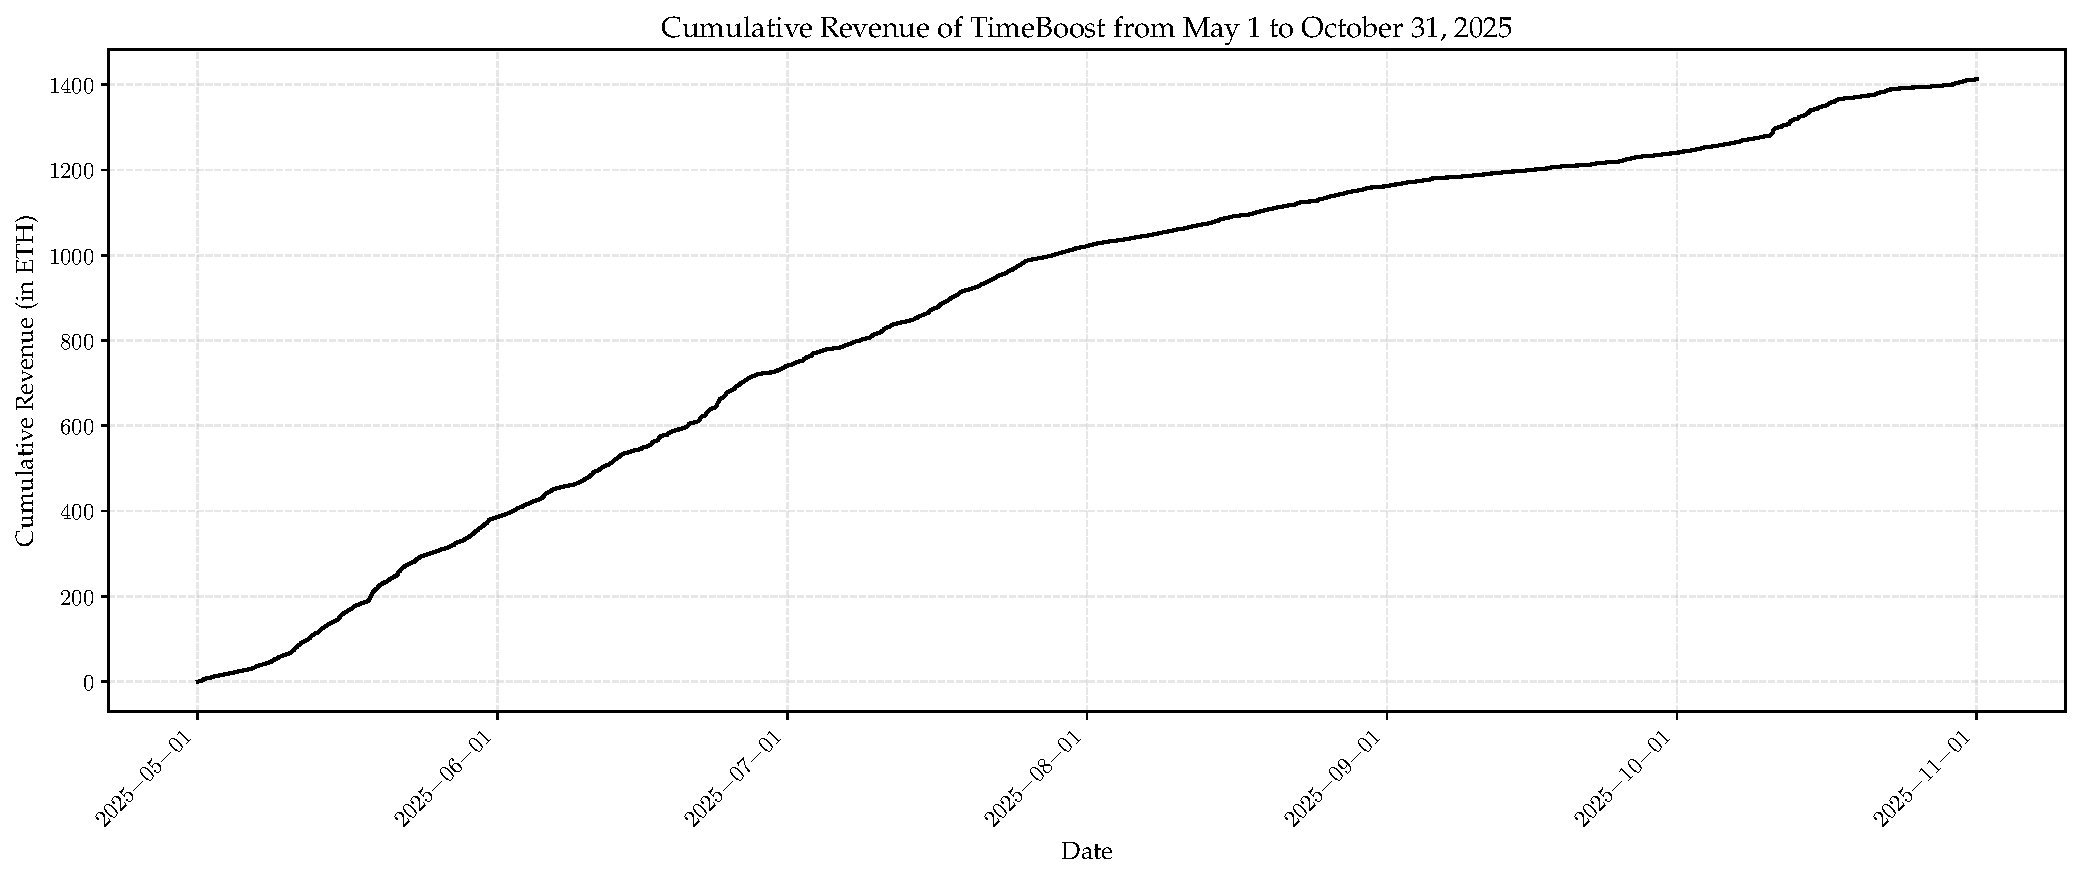
\includegraphics[width=0.8\linewidth]{images/cumulative_price.pdf}
    \caption{Cumulative revenue of Timeboost through express lane auction from May to October.}
    \label{fig:cumulative_price}
\end{figure}

\subsection{Related Literature}
% LVR and CEX-DEX Arbitrage
\paragraph*{Loss-versus-rebalancing and CEX-DEX Arbitrage.}
Following the foundational work of \cite{daian2019flash}, which introduced the term Maximal Extractable Value (MEV), a substantial body of literature has emerged exploring both its theoretical and empirical aspects. Early on, both academia and practitioners recognized CEX-DEX arbitrage as the primary source of MEV, commonly measured using short-term ($\le 5$ minutes) markouts \cite{wu2025measuring,gogol2024cross,heimbach2024non,oz2025pandora,followupuniv3,usageofmarkout}. Subsequently, \cite{milionis2022automated} provided a theoretical justification for such a metric and introduced Loss-Versus-Rebalancing (LVR), which has been generalized to more realistic settings in later works, including \cite{milionis2024automated} and \cite{nezlobin2025loss}. These studies, while differing in their specific details, consistently demonstrate a close relationship between CEX-DEX arbitrage and LVR, which represents the adverse selection cost borne by Automated Market Makers (AMMs). After abstracting away fees, gas costs, and inventory risk, the leading term of this relationship is shown to be $\bigO (\sigma^2)$, where $\sigma$ denotes the instantaneous volatility of the asset price.

% Timeboost, Theoretical and Empirical Works
\paragraph*{Time-based Transaction Ordering Policies and Timeboost.}
Even before the advent of blockchain technology, time-based transaction ordering policies and associated products were well established and widely adopted. For instance, since the late $2000$s, traditional finance (TradFi) exchanges have commercialized latency, offering ``speed technology'' to high-frequency trading (HFT) firms, generating revenues exceeding \$ $700$ million in $2017$ \cite{budish2024theory}. The impact of asymmetric speed bumps and micro-burst fees, exemplifying such exotic transaction ordering policies (priority rules), has been investigated by \cite{Aoyagi_2025} and \cite{brolley2023liquid}. Timeboost, as introduced in \cite{mamageishvili2023buying}, aligns with these policies, and \cite{akaki2025blind} and \cite{fritsch2024mev} provide a comprehensive theoretical understanding of its mechanisms. While Timeboost generated over $1400$ ETH in revenue from May to October, demonstrating its effectiveness, empirical research in this area remains nascent, with \cite{messias2025express} and \cite{mamageishvili2025timeboostaheadoftimeauctionswork} among the pioneering works that explore bidder behavior in ELA and the performance of Timeboost. In particular, the latter work claimed that the bidders' bids can be used as a noisy proxy for the markout of arbitrageurs' trades in the subsequent round.

% Variance Risk Premia
\paragraph*{Variance Risk Premia and Risk Aversion.}
A large body of literature documents a systematic wedge between the replication-based (risk-neutral) fair value of a variance swap and its traded price, commonly referred to as the variance (or volatility) risk premium (VRP). The ``fair'' strike for variance swap can be synthesized from an option strip \cite{demeterfi1999guide} or via model‐free implied variance \cite{jiang2005modelfree}, and the VRP is typically measured as implied minus subsequently realized variance ($\RV$) \cite{carr2009variance}. Empirically, this wedge is time-varying and (on average) negative, consistent with investors’ risk aversion and a stochastic nature of volatility that loads on variance and tail risks \cite{bakshi2003delta,bollerslev2009expected,broadie2007model,bollerslev2011tails}. Beyond level effects, the term structure and composition of premia matter as well: short-horizon variance premia are especially volatile and command higher compensation, and downside (``bad'') variance carries a larger premium than upside variance \cite{dewbecker2017price,aitsahalia2020term,feunou2018downside}. The phenomenon is not equity‐specific: analogous variance premia appear in foreign exchange (FX) and commodity markets, indicating a broad, asset-agnostic compensation for variance and jump risks \cite{londono2017fxvrp,prokopczuk2017commodityvrp,vantassel2018equityvrp}. Collectively, these results suggest that forward-looking prices for variance-linked payoffs can be persistently discounted relative to their ``fair'' values when risk is borne by risk-averse traders.

\subsection{Roadmap} % TODO: revise this paragraph
The subsequent sections of this paper are structured as follows: Section 2 provides a theoretical foundation for the proposed model and hypothesis. Section 3 outlines the data sources and the analytical methodologies employed, presents results, and discusses the findings and their implications. The paper concludes with Section 4, which summarizes the key findings and potential future research topics.